\chapter{UML modeling}
\label{cha:modeling}

\section{Use Case}
\subsection{Create Appointment}
\begin{center}
	\begin{tabular}{|c||p{0.6\textwidth}|}
		\hline
		Name & Create appointment \\ \hline
		Actors & User \\ \hline
		Assumption & The user need to insert a new appointment in his personal calendar \\ \hline
		Pre-Conditions & \begin{itemize}
			\item The user has successfully signed to the system
			\item The user has already opened the window with the insertion form.
		\end{itemize} \\ \hline
		Flow of events & \begin{enumerate}
			\item The user creates a new appointment by inserting all the information needed in order to adding a new event correctly in his own calendar.
			\item The system check into the calendar if the location of the appointment is reachable in the allotted time or if the event is overlapping with other appointment.
			\item The user is informed by a warning message about the actual validation of the appointment.
			\item The user have to confirm o reject the insertion of the appointment
		\end{enumerate} \\ \hline
		Post-Conditions & The appointment of the user has been stored to the system in the event that he has confirmed the inclusion. \\ \hline
		Exception & An internal system error makes impossible to store the reservation data. The user is notified of the error \\ \hline		
	\end{tabular}
\end{center}

\begin{figure}
	\centering
	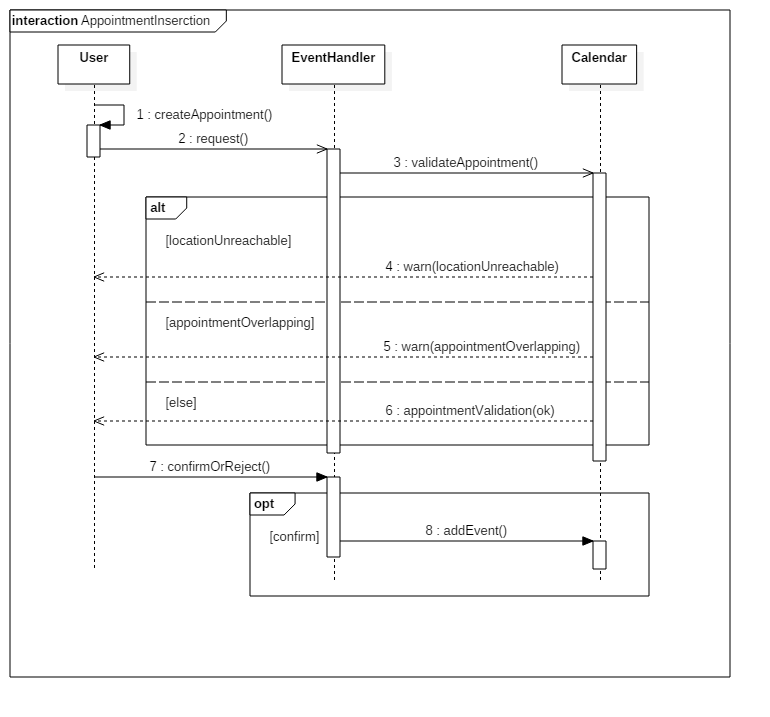
\includegraphics[width=6in]{./diagrams/AppointmentInserction.png}
	\caption{Sequence Diagram: Create Appointment}
	\label{fig:SequenceAddApp}
\end{figure}



